\documentclass[11pt]{article}
\usepackage[margin=1in]{geometry}

\usepackage{amsmath}
\usepackage{amssymb}
\usepackage[utf8]{inputenc} 
\usepackage{graphicx} 
\usepackage{parskip} 
\usepackage{multirow} 
\usepackage{mathtools}

\DeclarePairedDelimiter\abs{\lvert}{\rvert}%
\DeclarePairedDelimiter\norm{\lVert}{\rVert}%

\makeatletter
\let\oldabs\abs
\def\abs{\@ifstar{\oldabs}{\oldabs*}}

\let\oldnorm\norm
\def\norm{\@ifstar{\oldnorm}{\oldnorm*}}
\makeatother
\usepackage{multicol} 
\usepackage[spanish,es-nodecimaldot]{babel} 
\usepackage{mathtools}
\usepackage{amsfonts}
\usepackage{float}
\usepackage{textcomp}
\usepackage{caption}
\usepackage{subfig}
\usepackage[spanish]{babel}
\usepackage{gensymb}
\def\sen{\mathop{\mbox{\normalfont sen}}\nolimits}

\usepackage{fancyhdr}
\fancyhf{}
\rfoot{\thepage}
\pagestyle{fancy}
\lhead{Nieto Castellanos Jaime Fabián}
\chead{}
\rhead{Tarea 5. Histogramas}
\begin{document}
Elegimos los eventos que corresponden a las entradas 6,944; 17,310;  13,773;  30,719; 24,809, para buscar cascadas atmosféricas, puesto que como se puede revisar en el archivo de datos, trig\_ run009776\_ 00692.root, estos eventos contienen más de 500 hits de 2 y 4 edges. 

\textbf{Problema 1)}

\begin{figure}[H]
\centering
\subfloat[Número de evento: 6944]{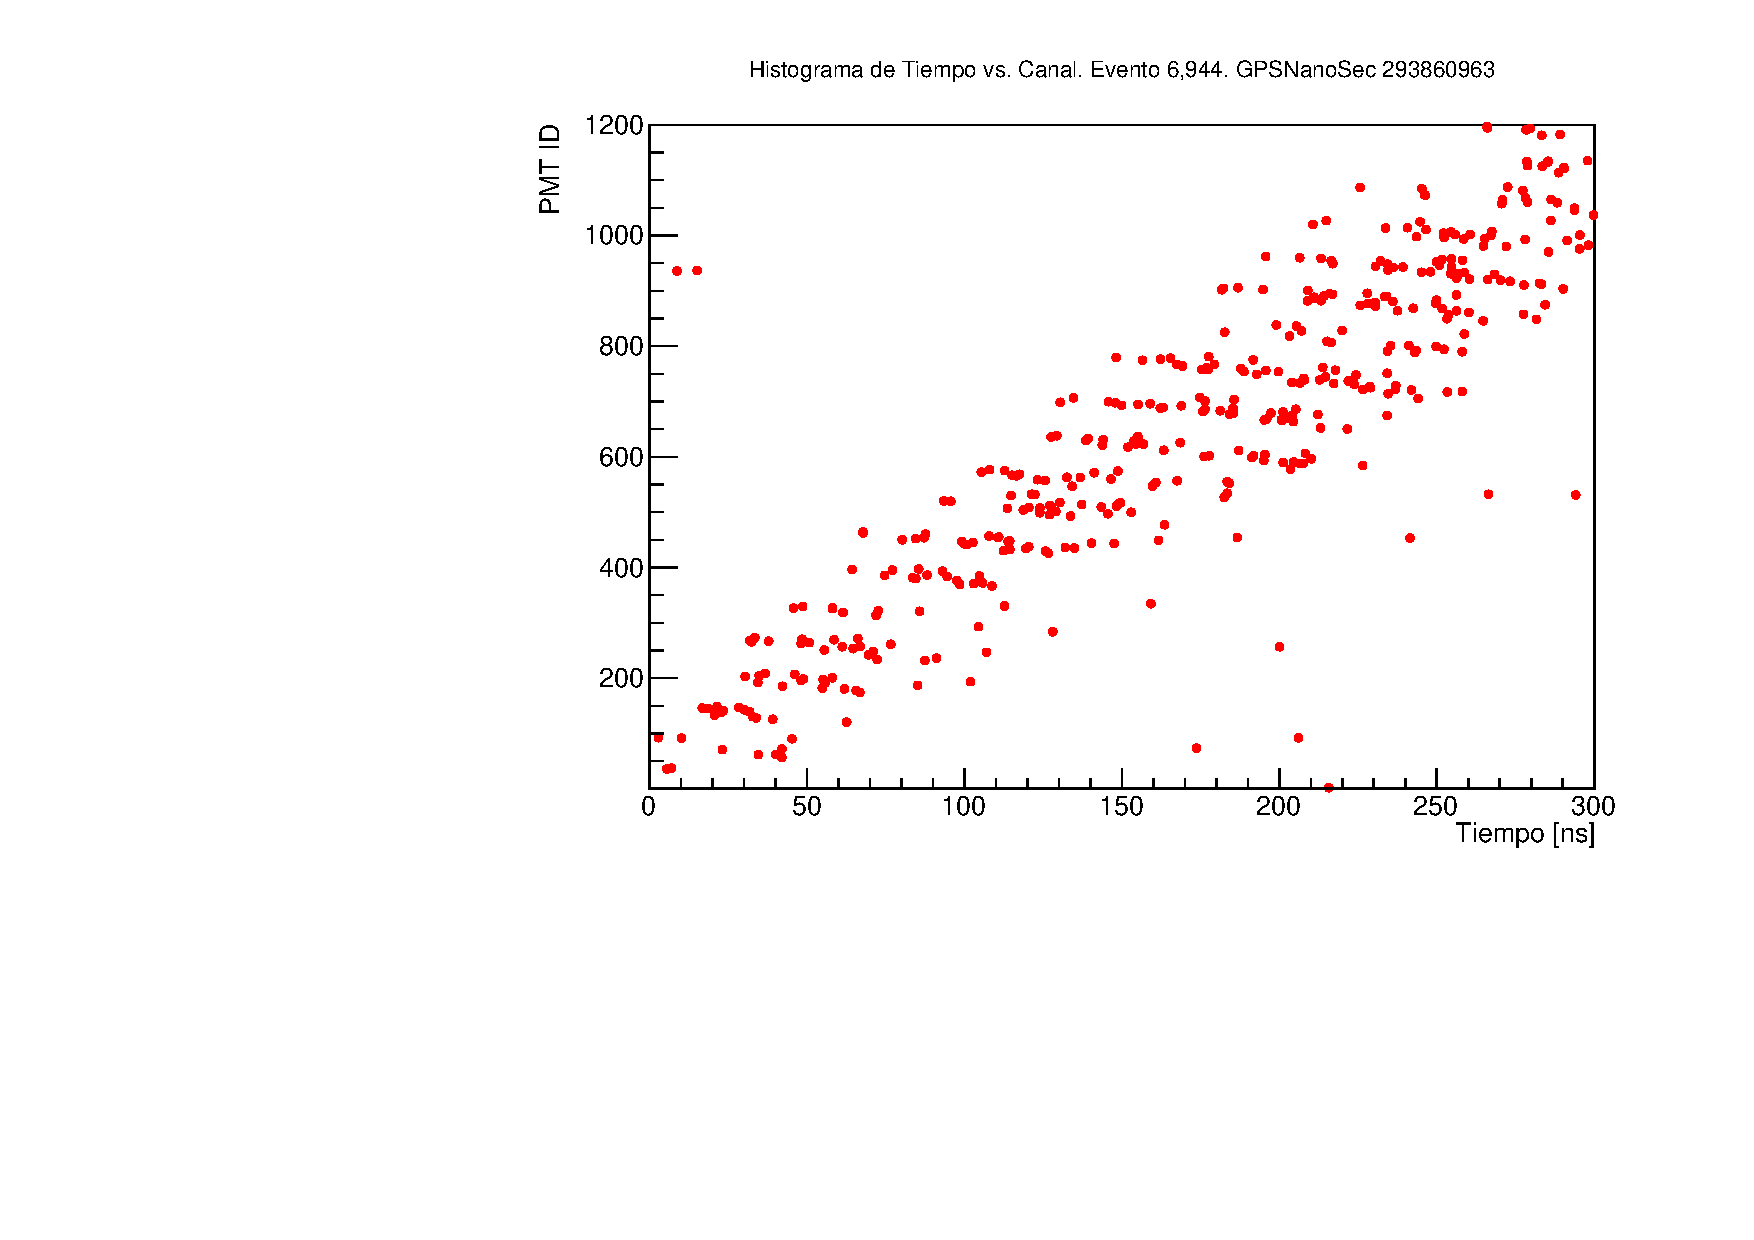
\includegraphics[width=0.5\textwidth]{../Figuras/Prob1HistEv1}}\subfloat[Número de evento: 17,310]{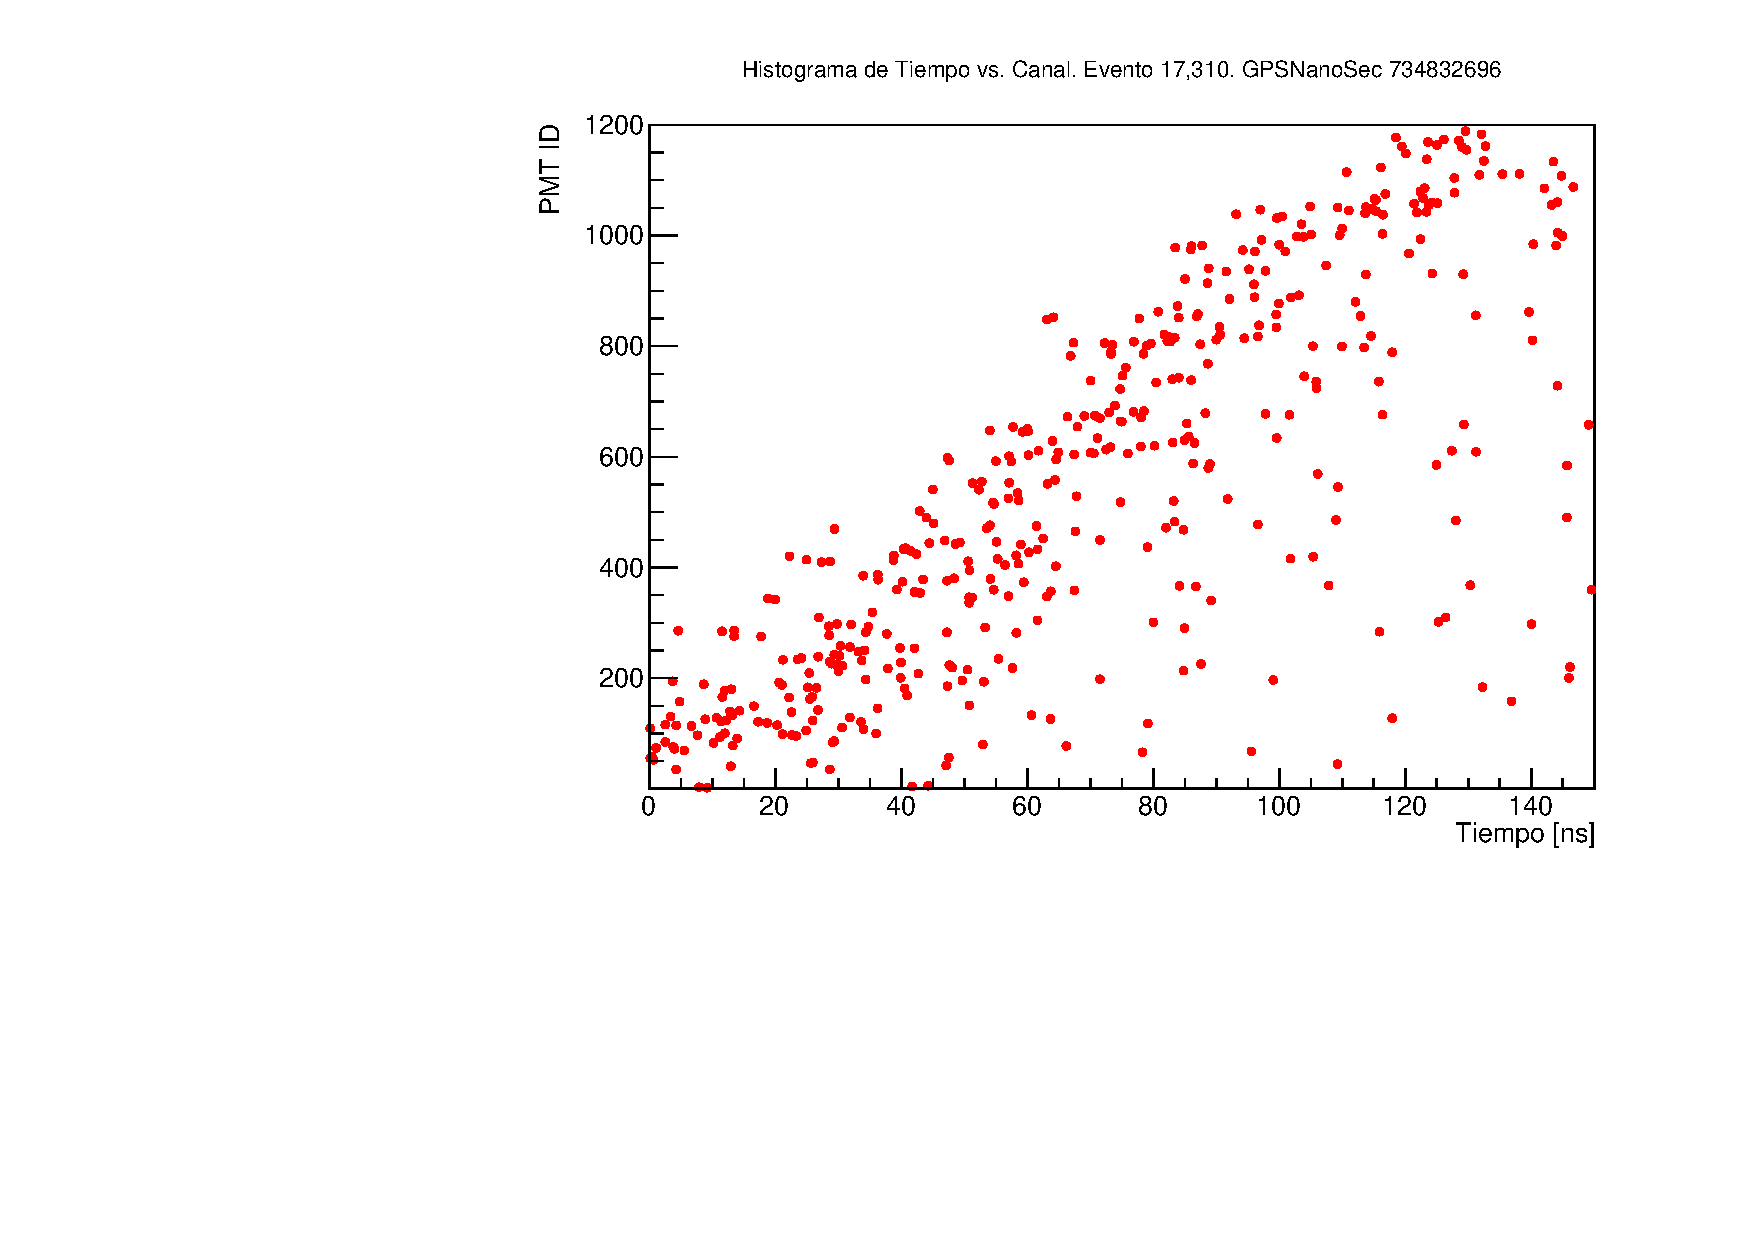
\includegraphics[width=0.5\textwidth]{../Figuras/Prob1HistEv2}}

\subfloat[Número de evento: 13,773]{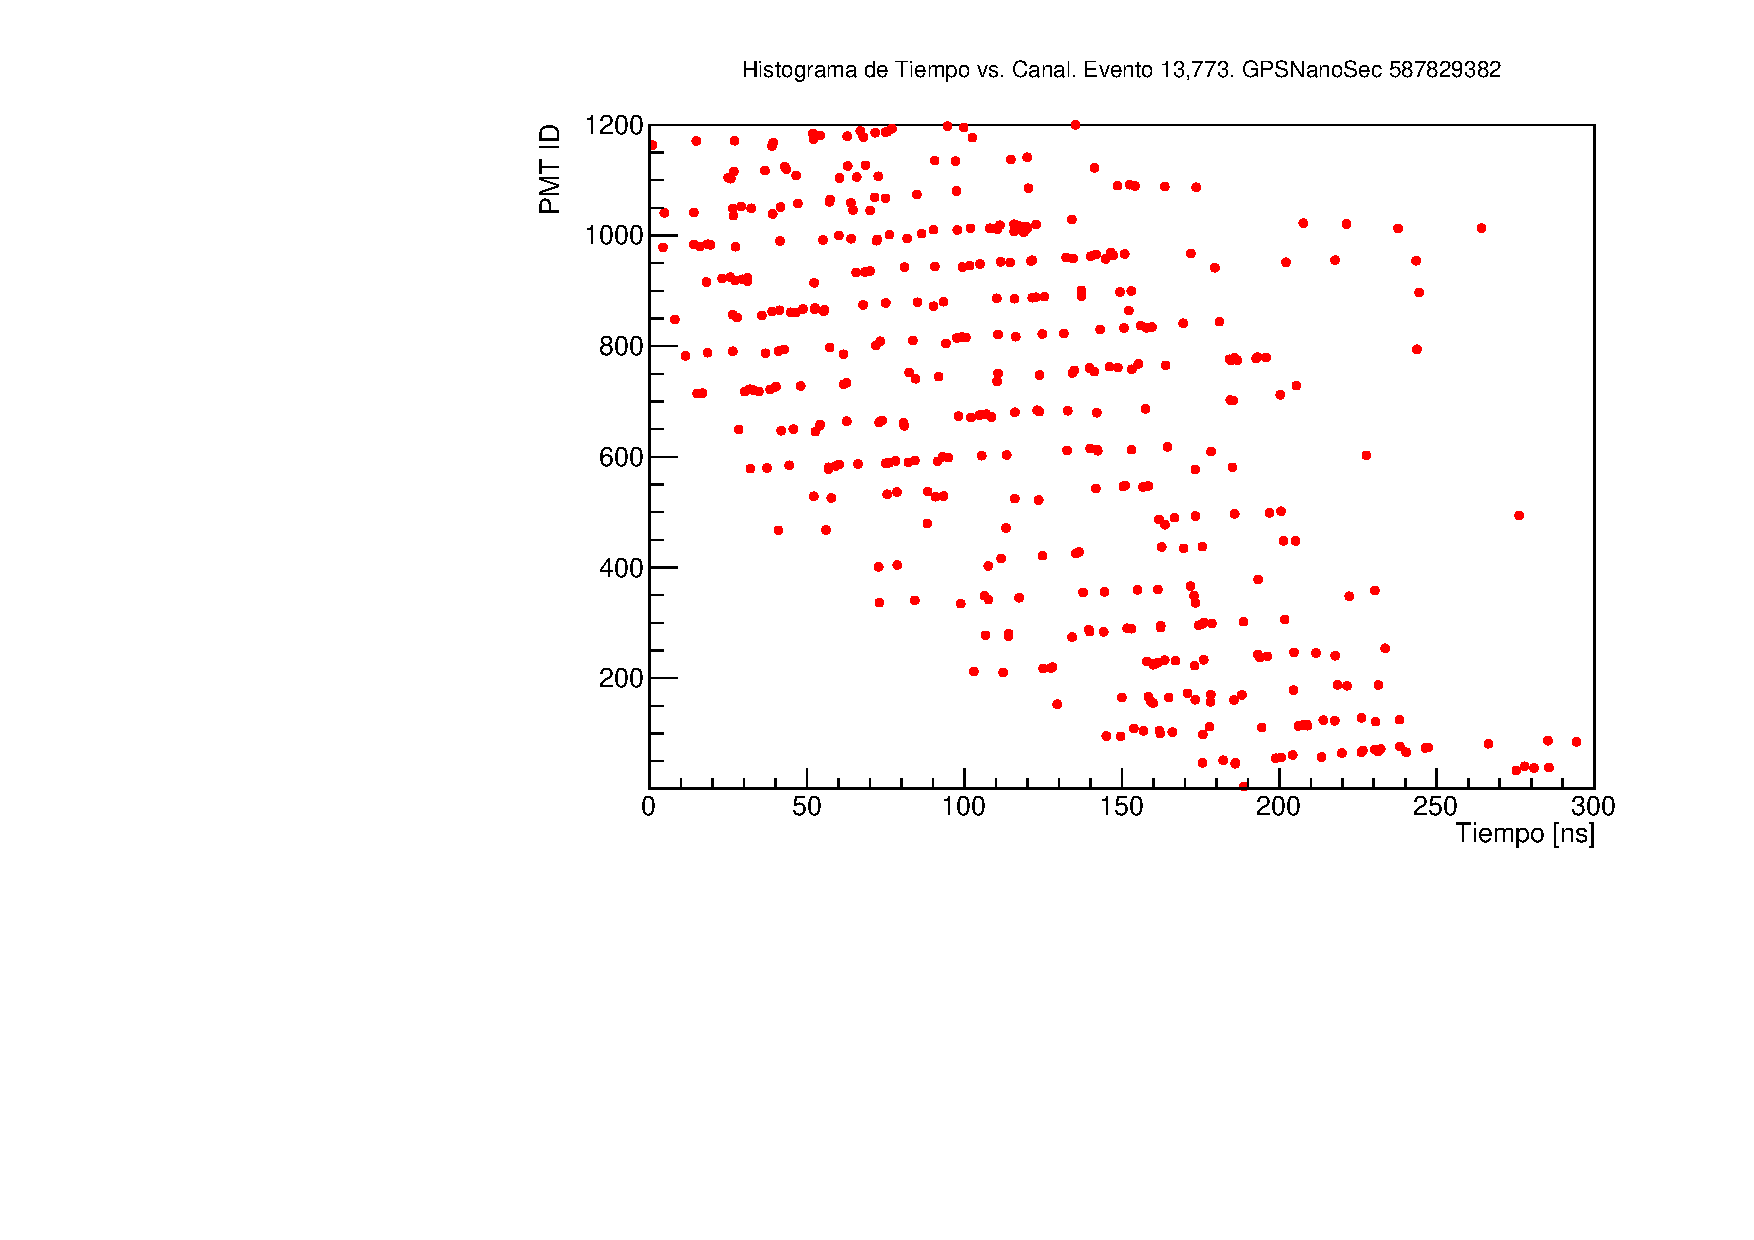
\includegraphics[width=0.5\textwidth]{../Figuras/Prob1HistEv3}}\subfloat[Número de evento: 30,719]{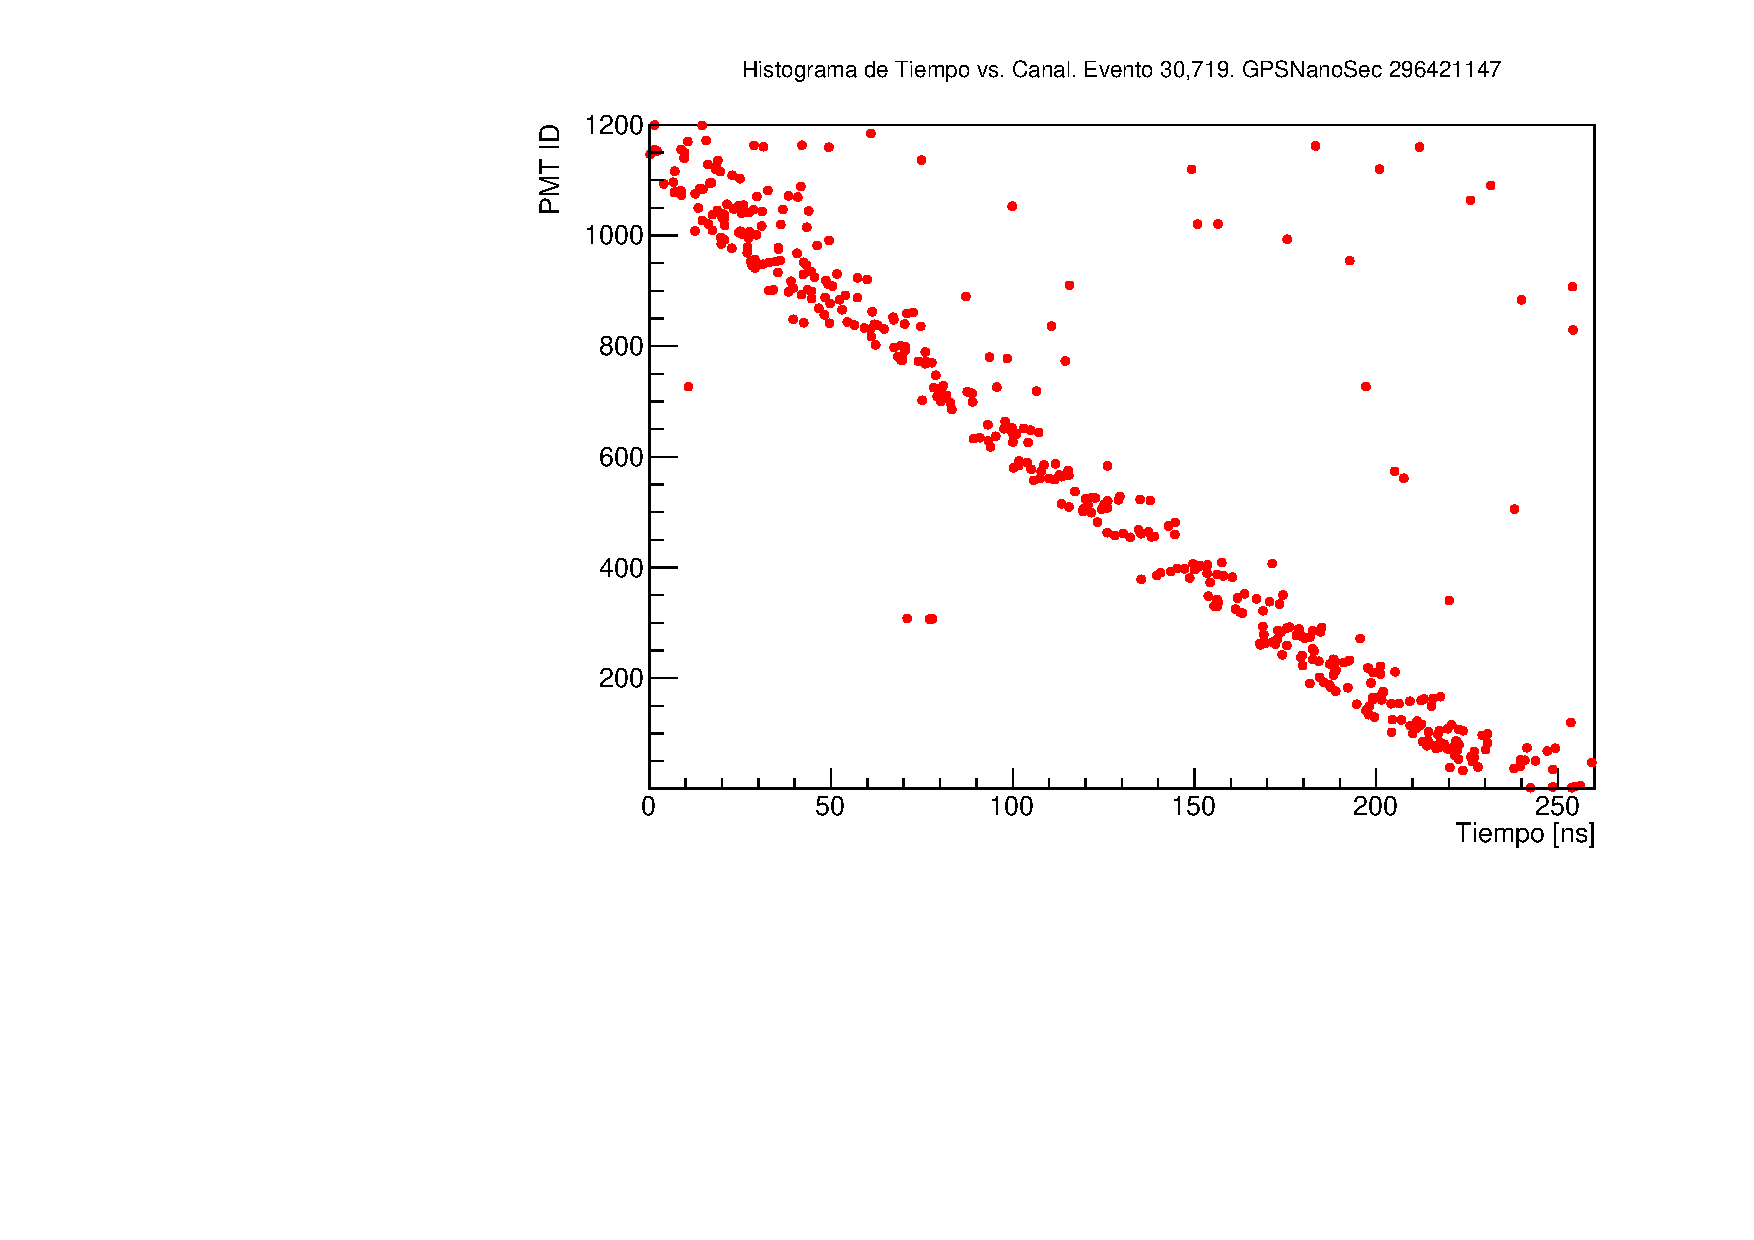
\includegraphics[width=0.5\textwidth]{../Figuras/Prob1HistEv4}}

\subfloat[Número de evento: 24,809]{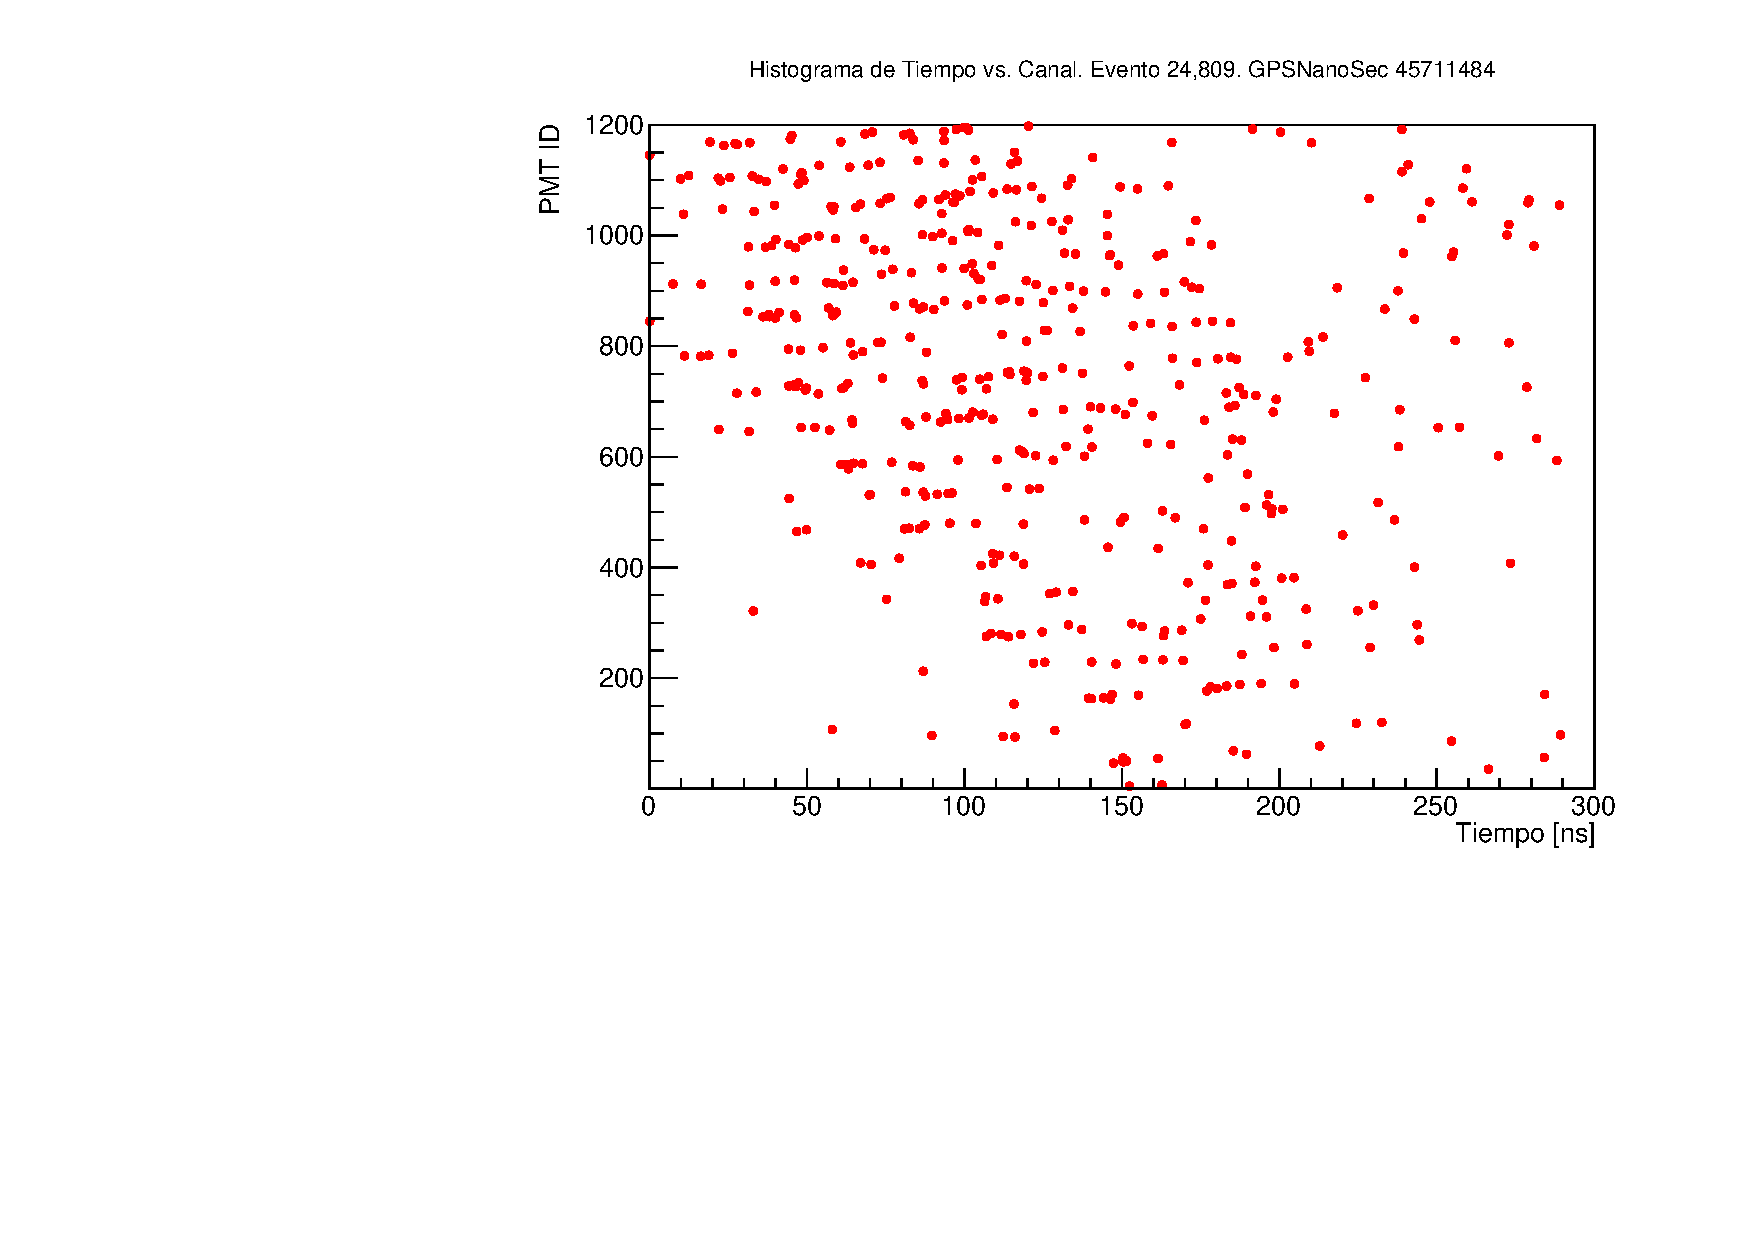
\includegraphics[width=0.5\textwidth]{../Figuras/Prob1HistEv5}}

\caption{Histogramas de tiempo vs. PMT ID para distintos eventos en donde se muestran cascadas atmosféricas.}
\label{fig:Prob1}
\end{figure}

\pagebreak
\textbf{Problema 2)}
Elegimos los eventos correspondientes a las entradas 13,773 y 24,809 del árbol de datos para hacer la comparación al aplicar el corte de calidad.

\begin{figure}[H]
\centering
\subfloat[Evento 13,773 sin corte de calidad]{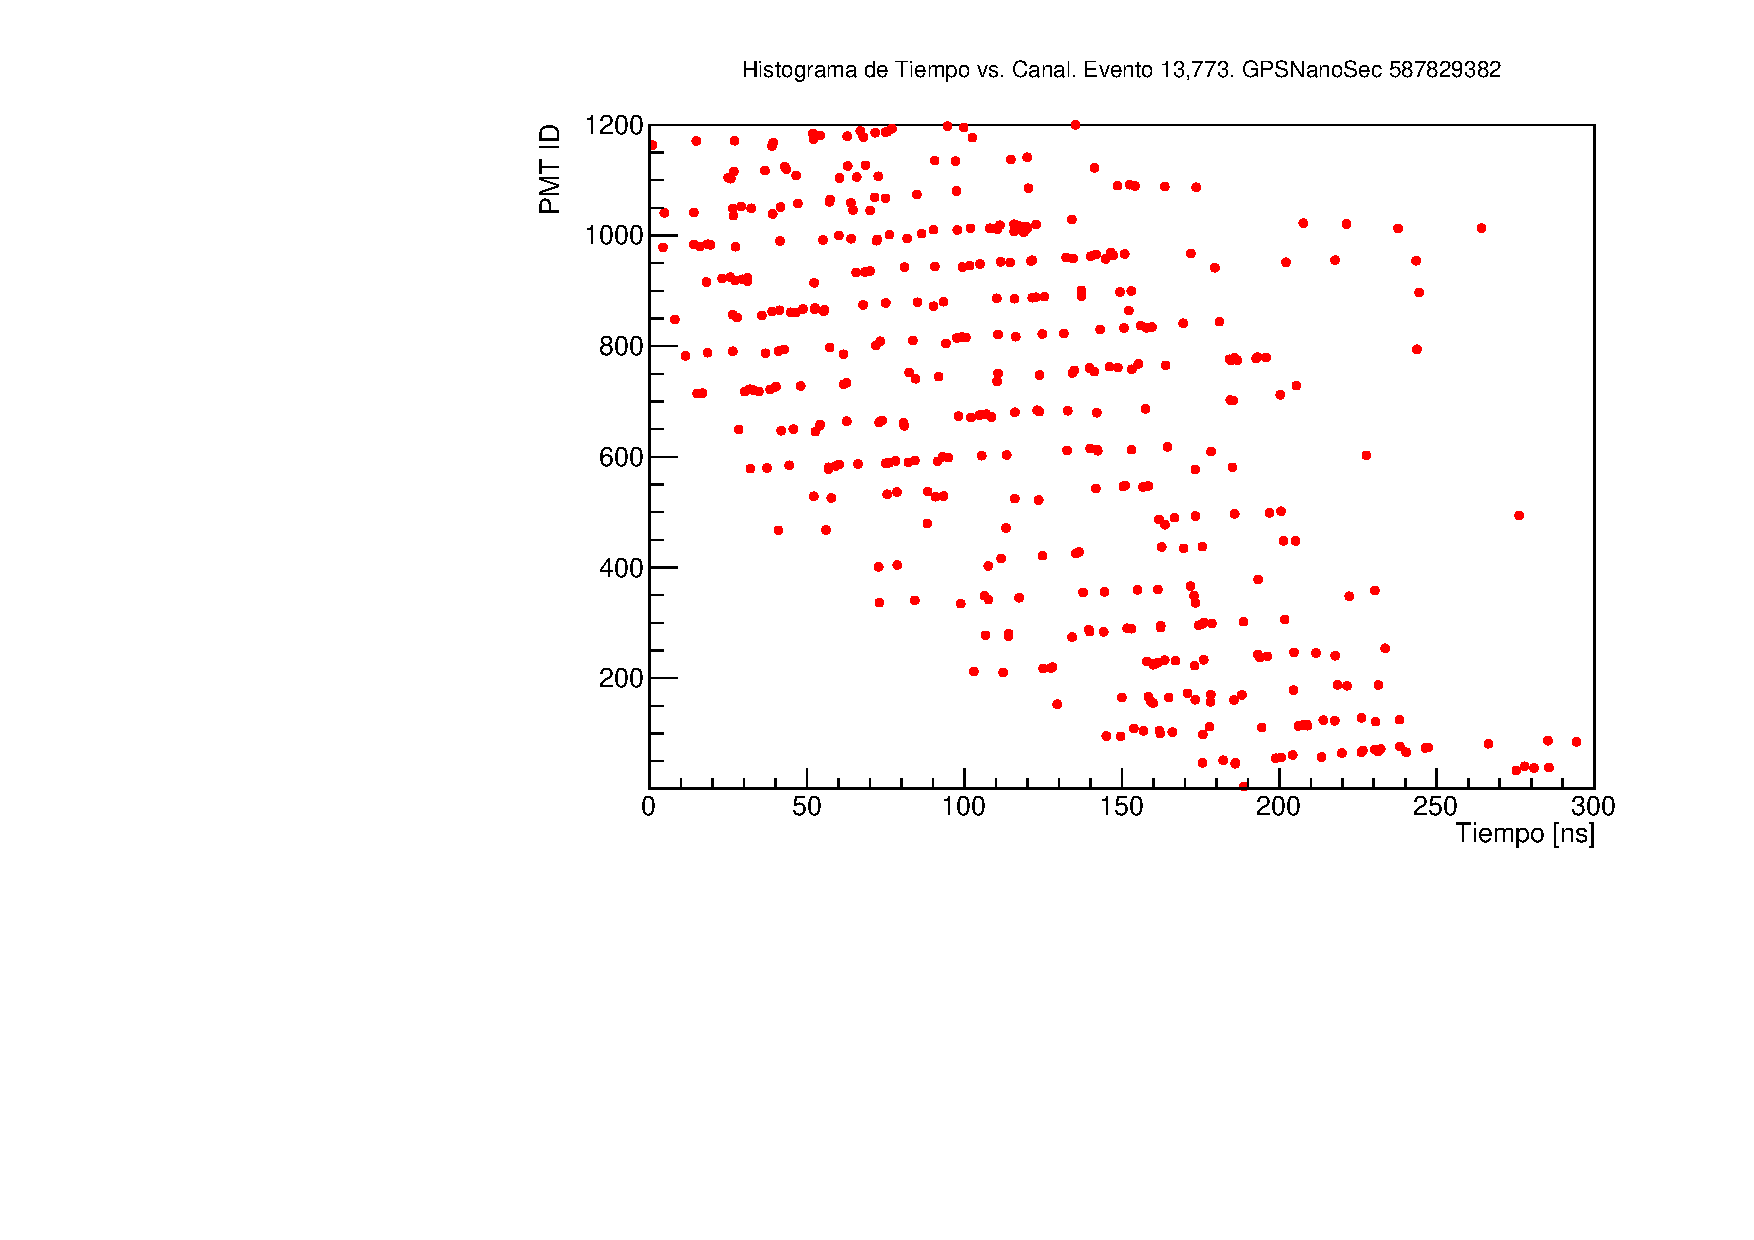
\includegraphics[width=0.5\textwidth]{../Figuras/Prob1HistEv3}}\subfloat[Evento 13,773 con corte de calidad]{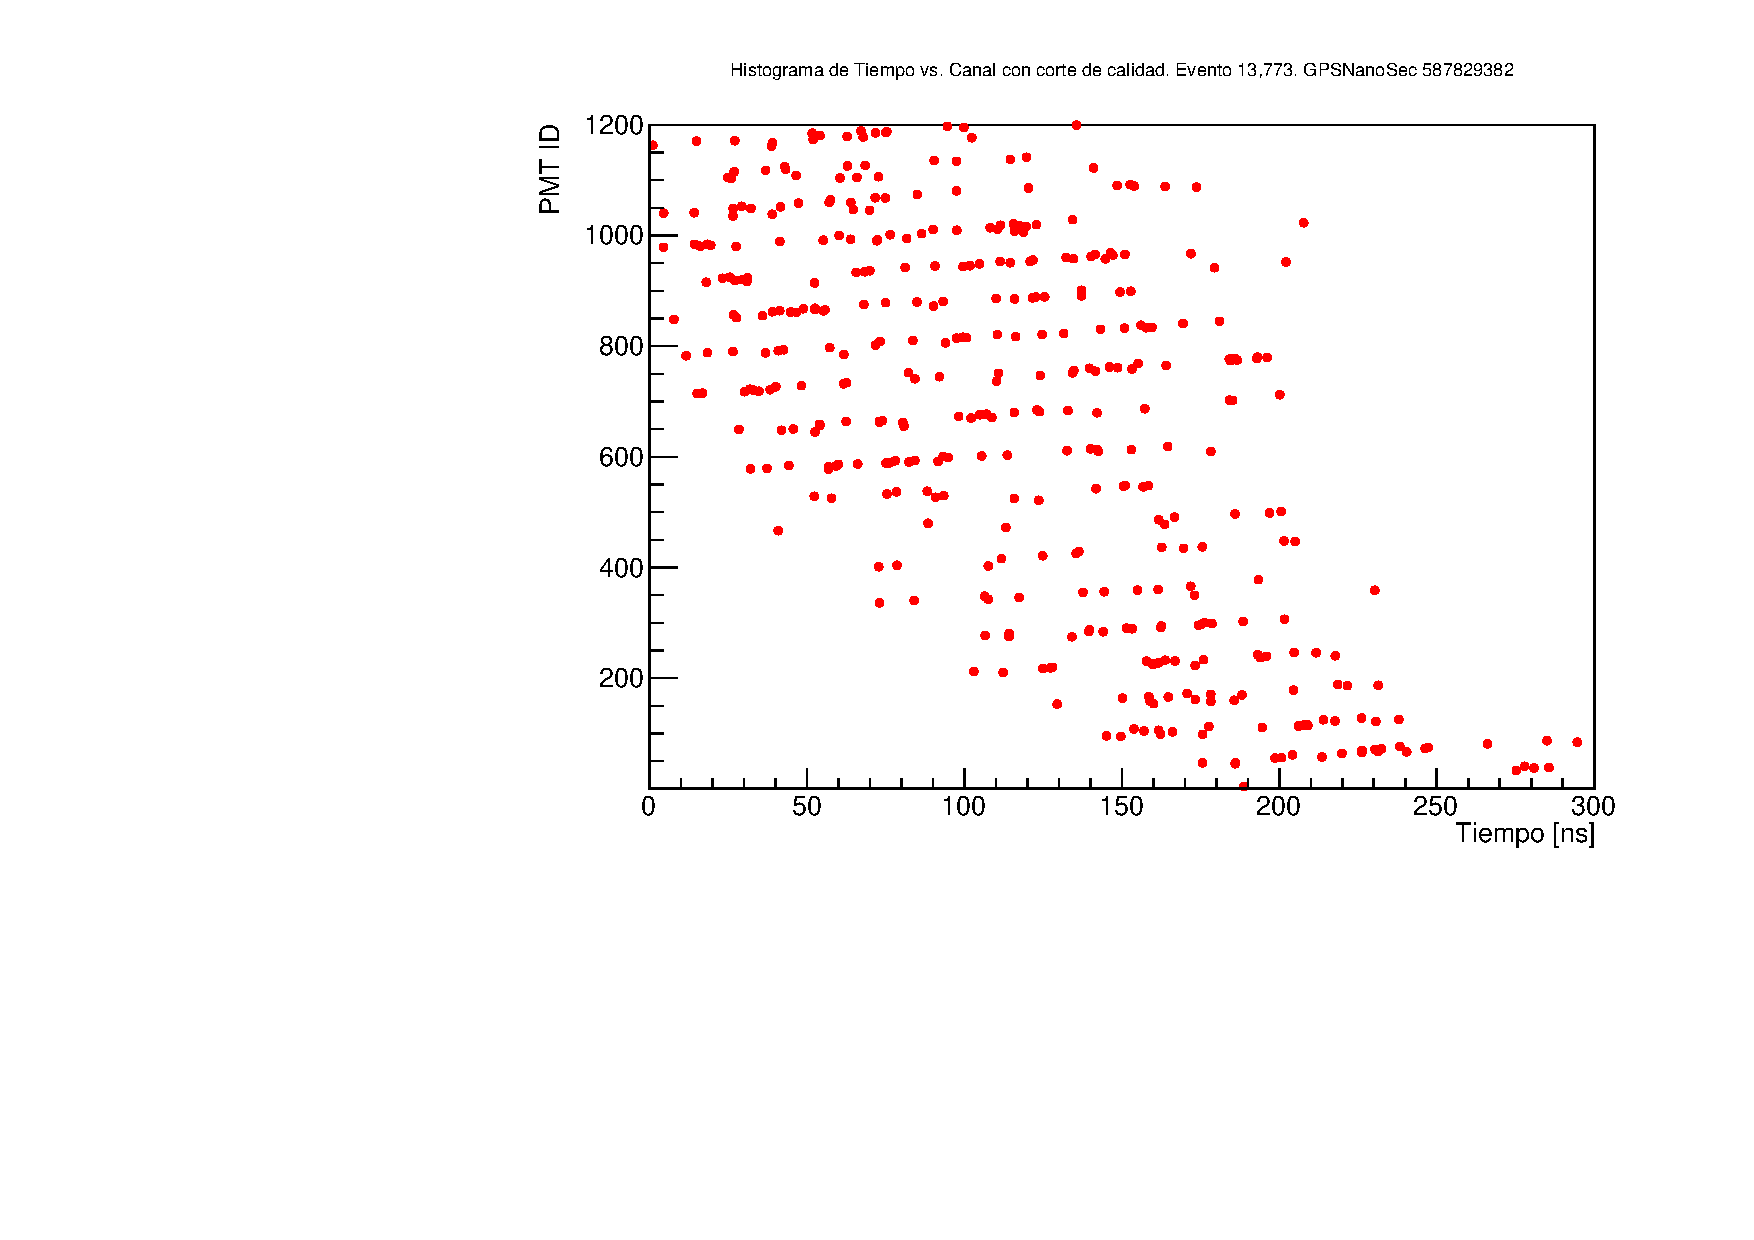
\includegraphics[width=0.5\textwidth]{../Figuras/Prob2HistEv1}}

\subfloat[Evento 24,809 sin corte de calidad]{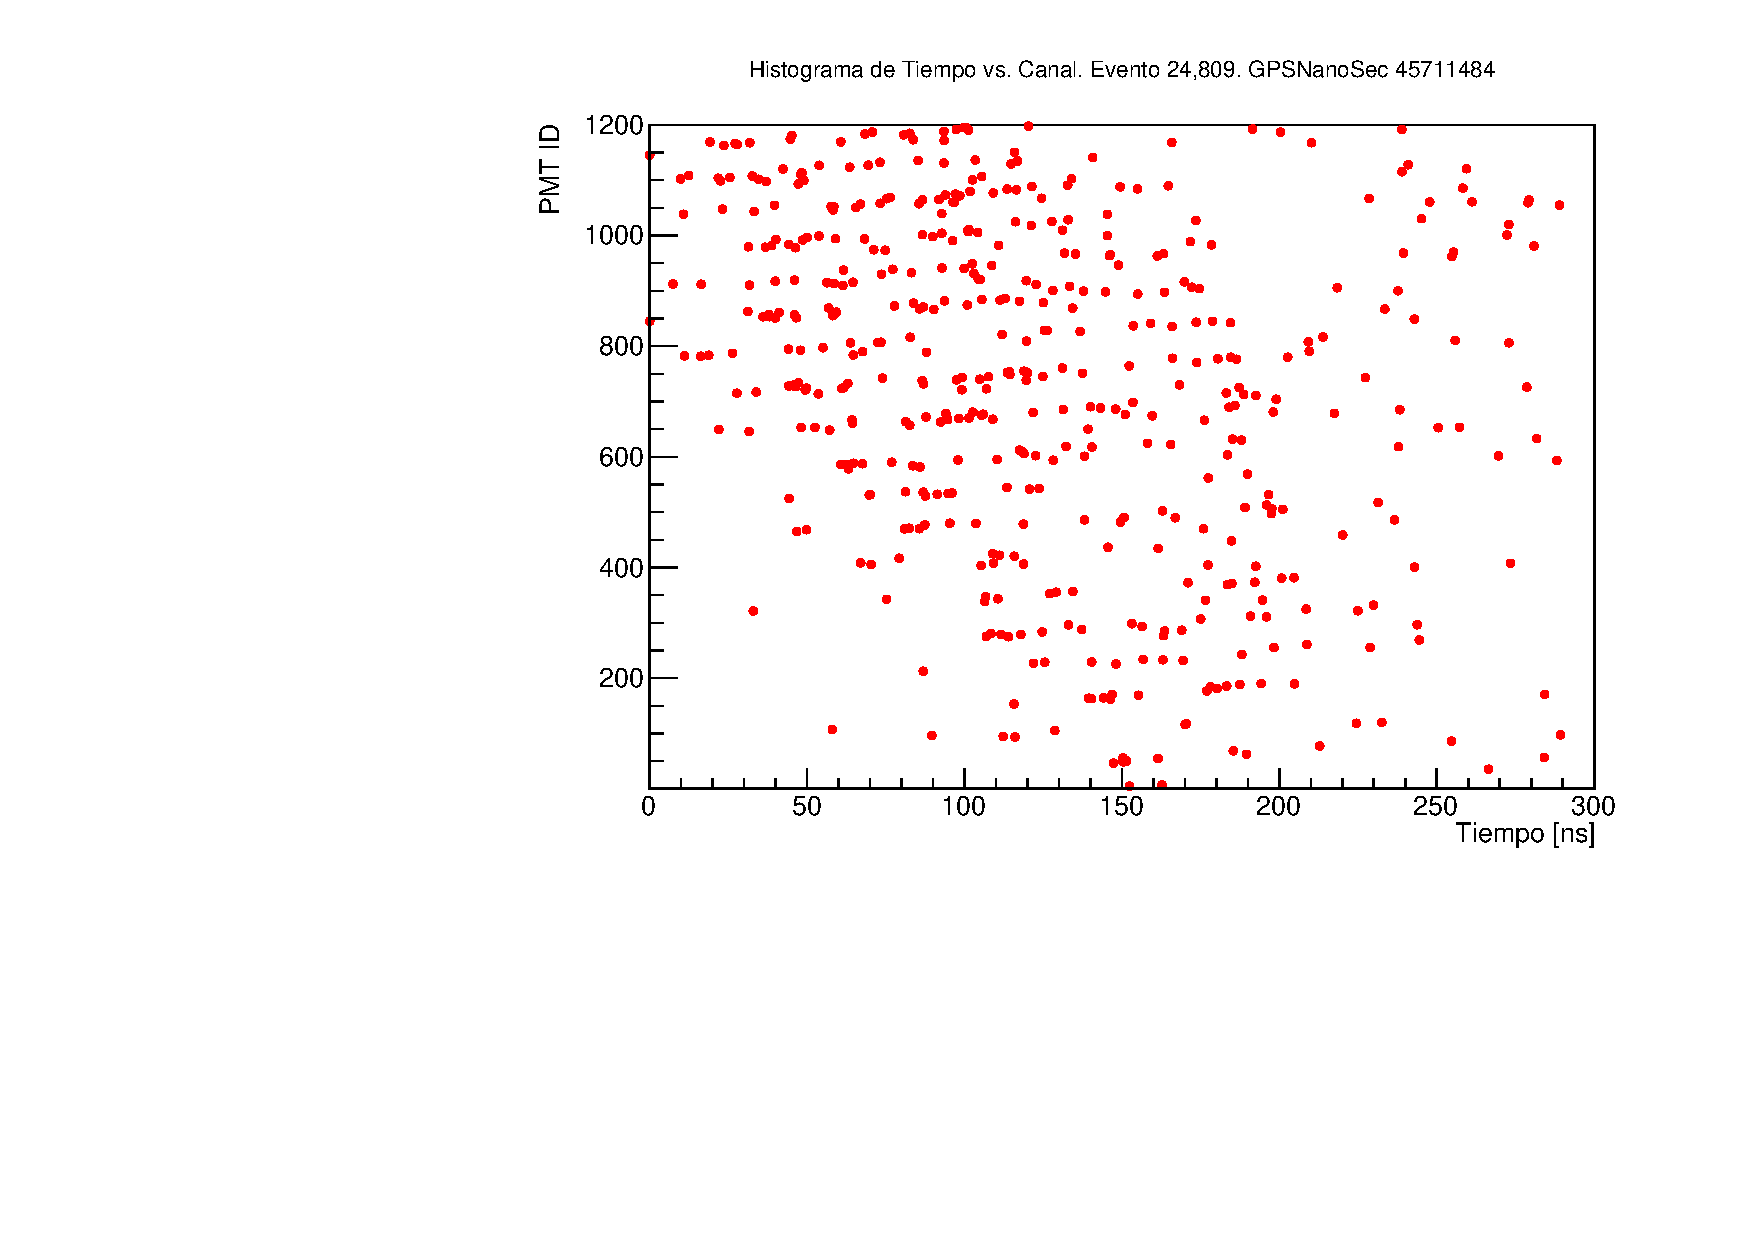
\includegraphics[width=0.5\textwidth]{../Figuras/Prob1HistEv5}}\subfloat[Evento 24,809 con corte de calidad]{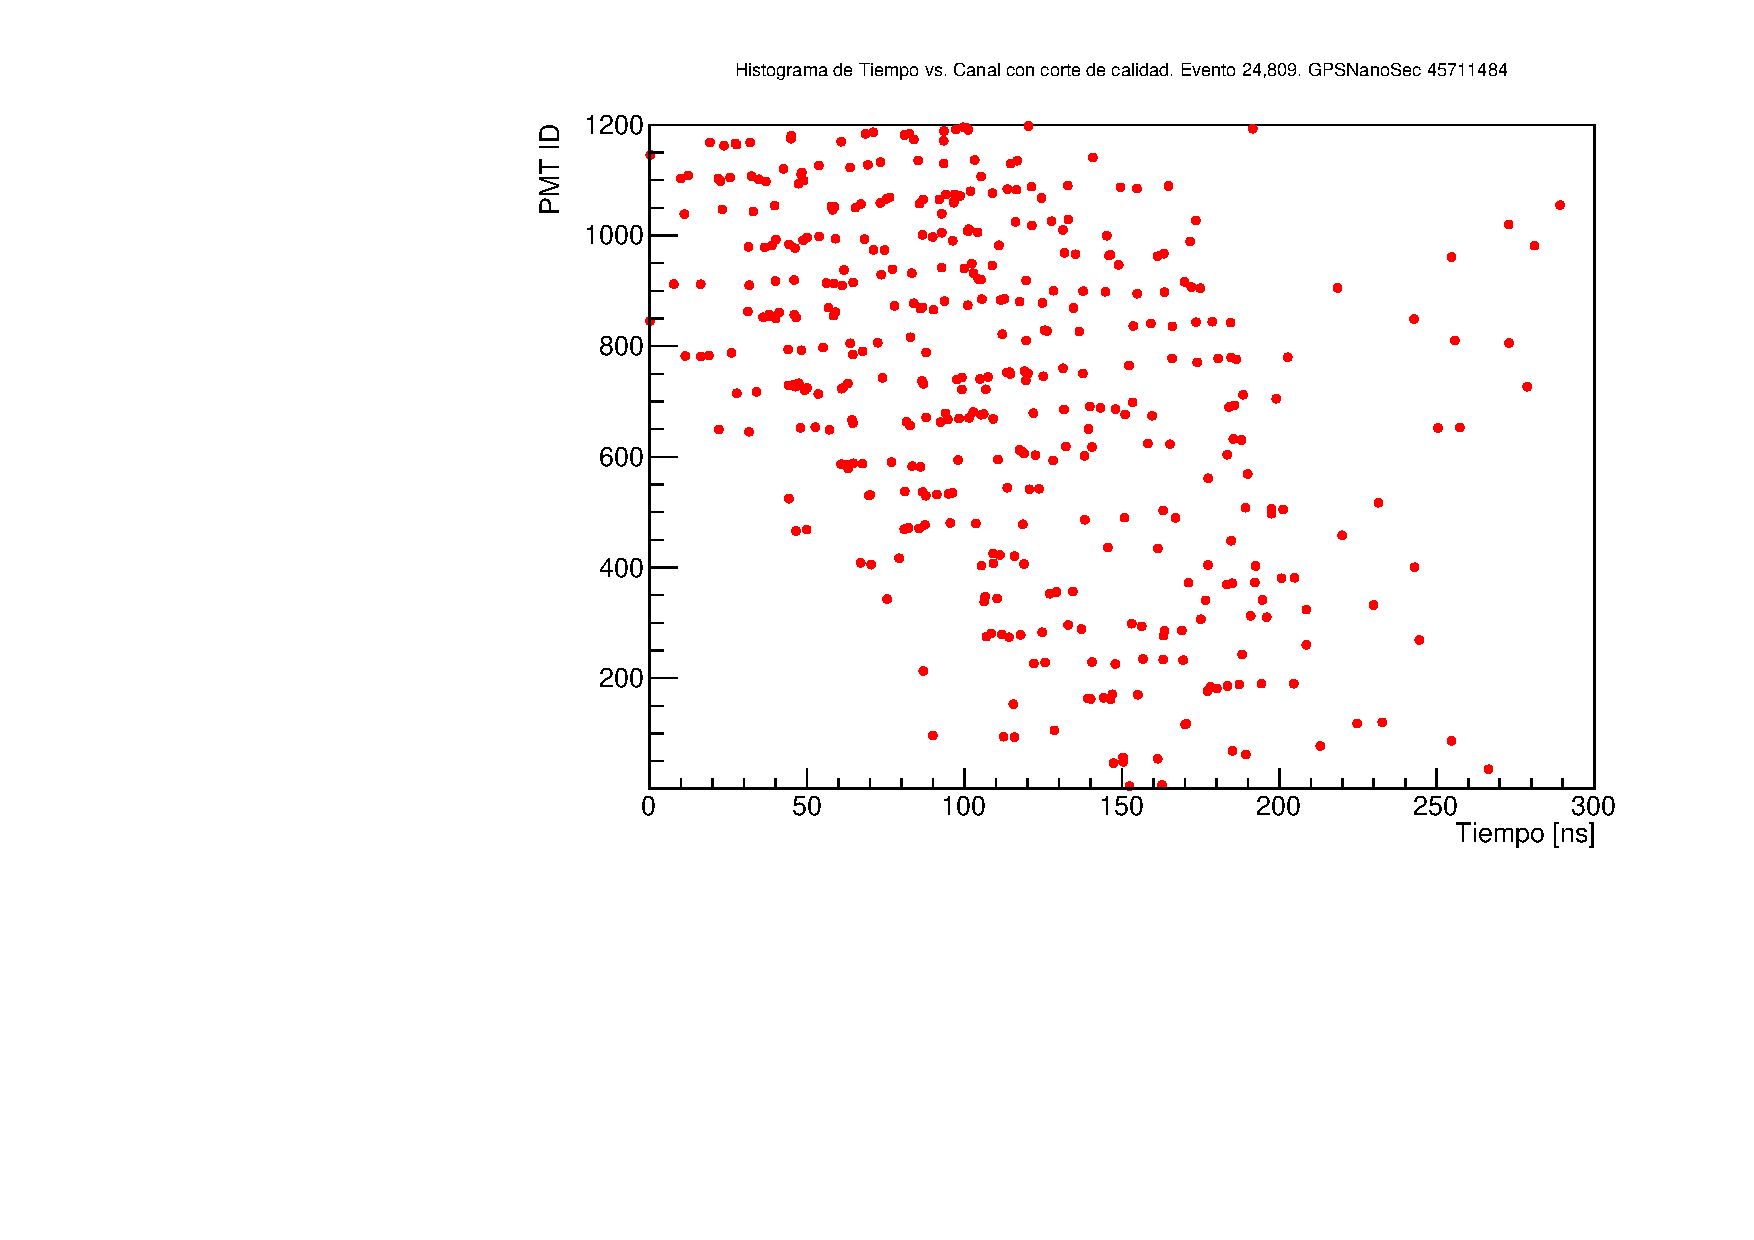
\includegraphics[width=0.5\textwidth]{../Figuras/Prob2HistEv2}}
\caption{Comparación de las cascadas atmosféricas detectadas en dos eventos distintos con y sin corte de calidad}
\label{fig:Prob2}
\end{figure}
\pagebreak


\textbf{Problema 3)}
\begin{figure}[H]
\centering
\subfloat[Número de eventos vs. frecuencia de hits de 2 edges]{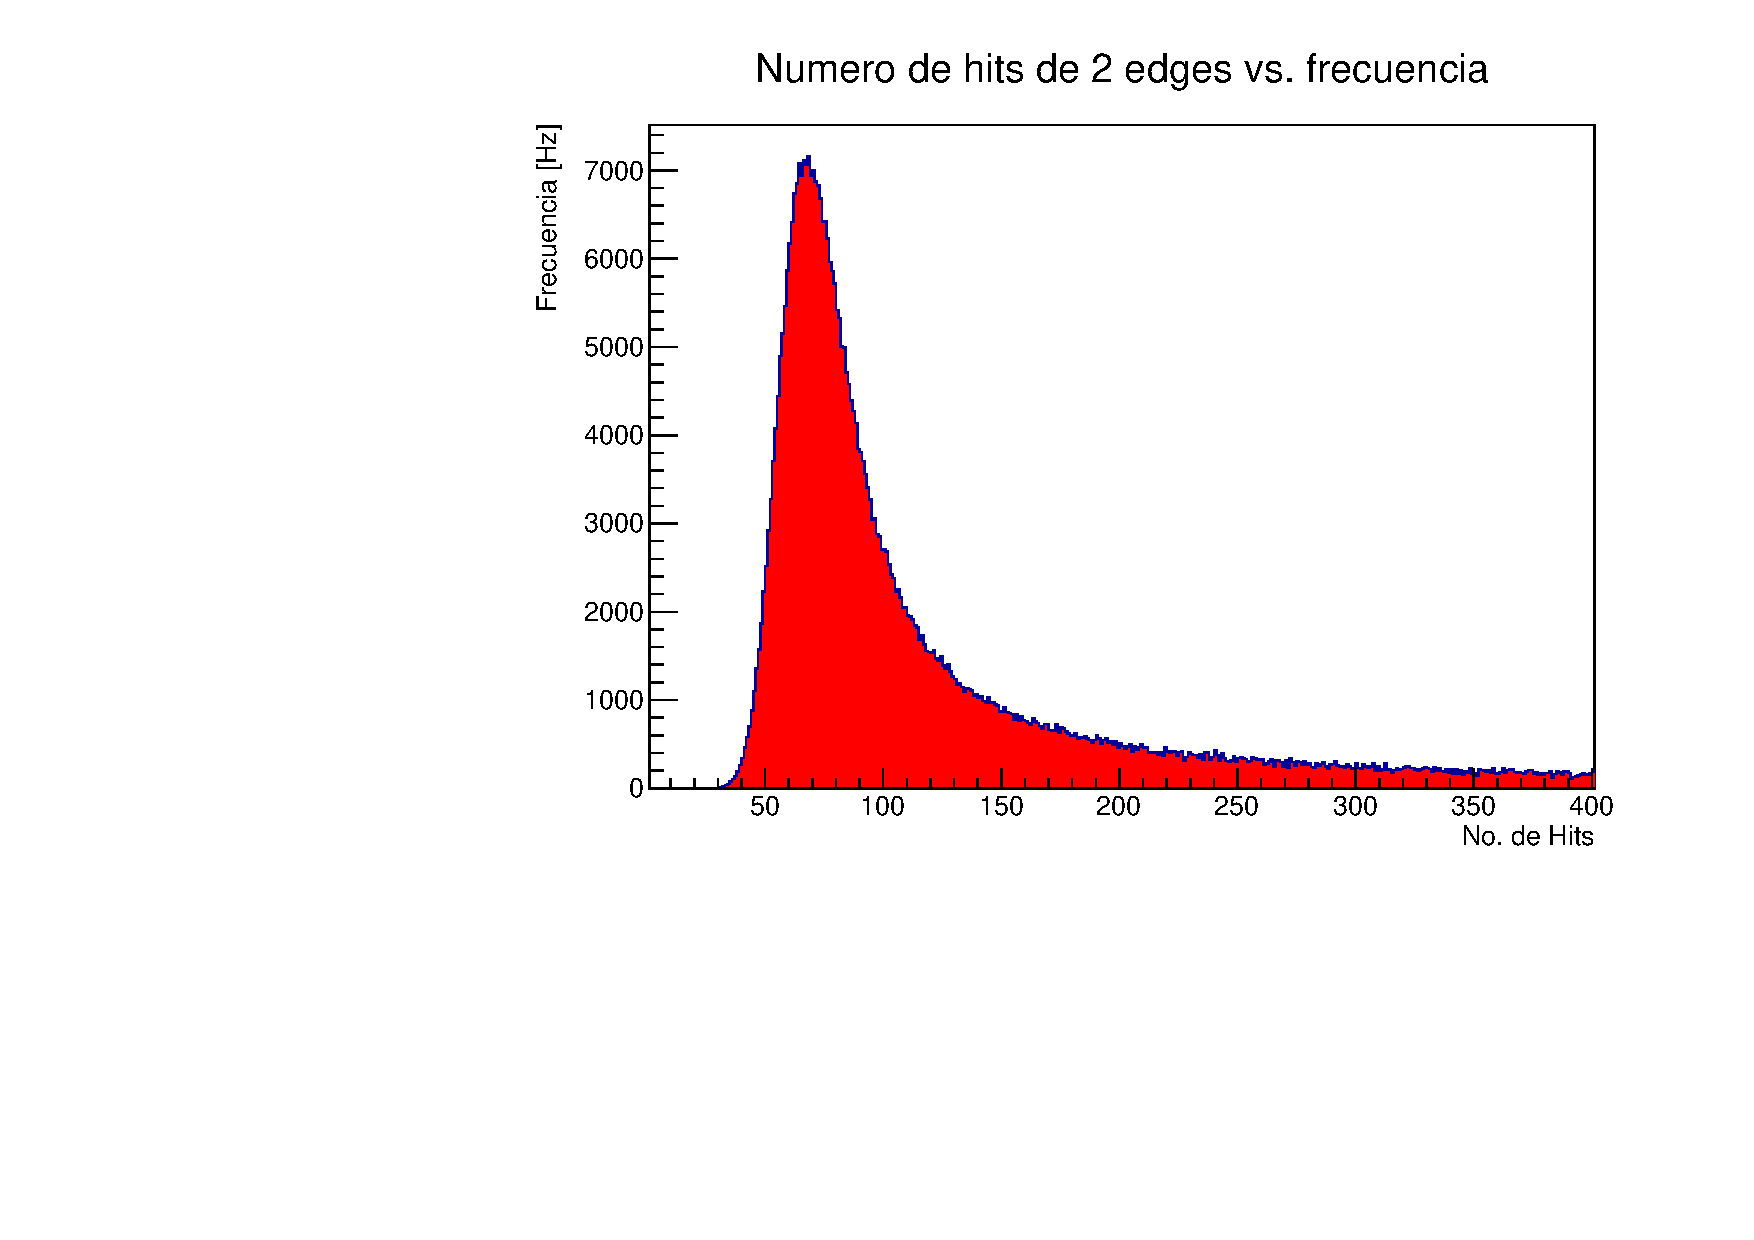
\includegraphics[width=0.55\textwidth]{../Figuras/Prob32Edge}}\subfloat[Número de eventos vs. frecuencia de hits de 4 edges]{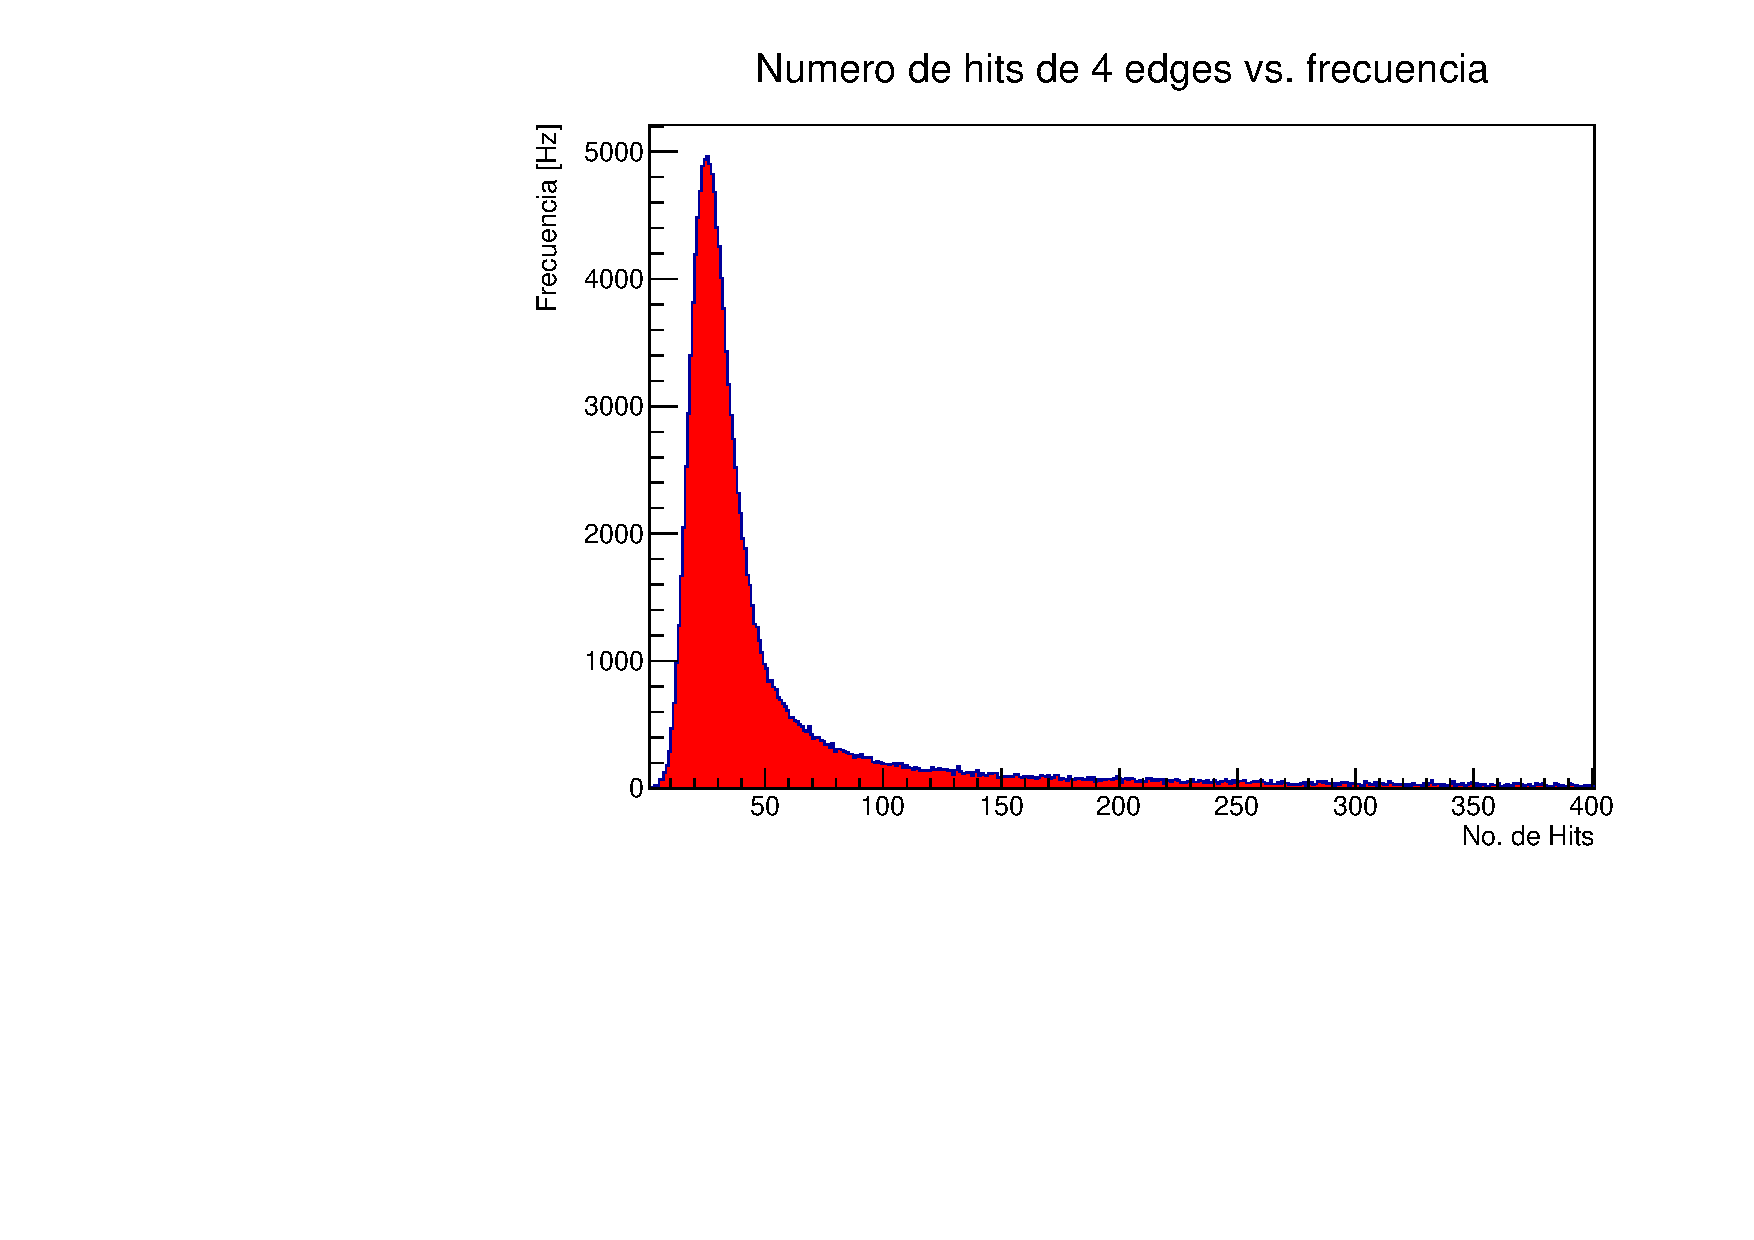
\includegraphics[width=0.55\textwidth]{../Figuras/Prob34Edge}}

\subfloat[Número de eventos vs. frecuencia de hits de 2 y 4 edges]{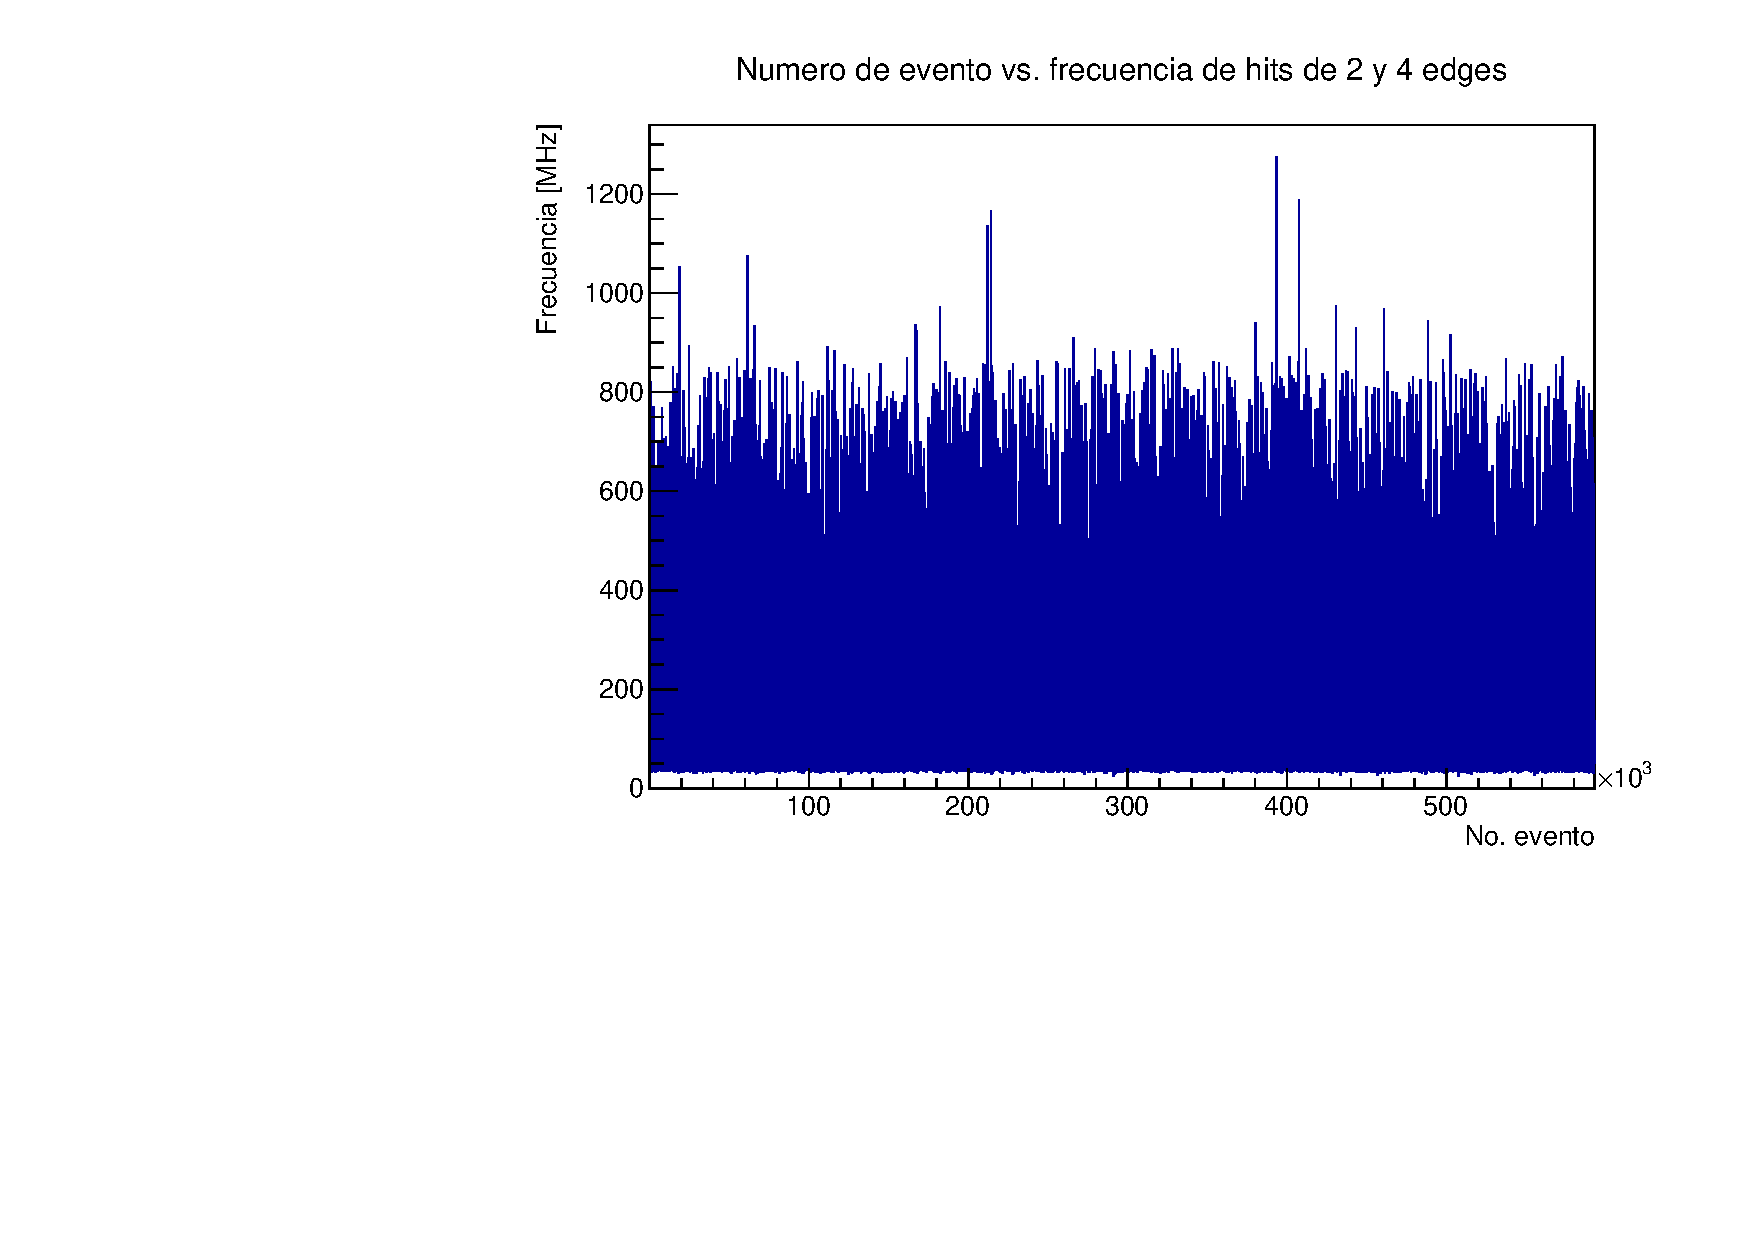
\includegraphics[width=0.55\textwidth]{../Figuras/Prob32y4Edge}}
\caption{En los histogramas se muestra el número de hits, de 2 y 4 edges, que fueron usados para el trigger (trigger flag=1), así como el número de hits que no fueron usados para el trigger (trigger flag=0).}
\label{fig:Prob3}
\end{figure}


\pagebreak

\textbf{Problema 4)}

\begin{figure}[H]
\centering
\subfloat[Trigger flag vs. PMT ID para hits con 2 edges]{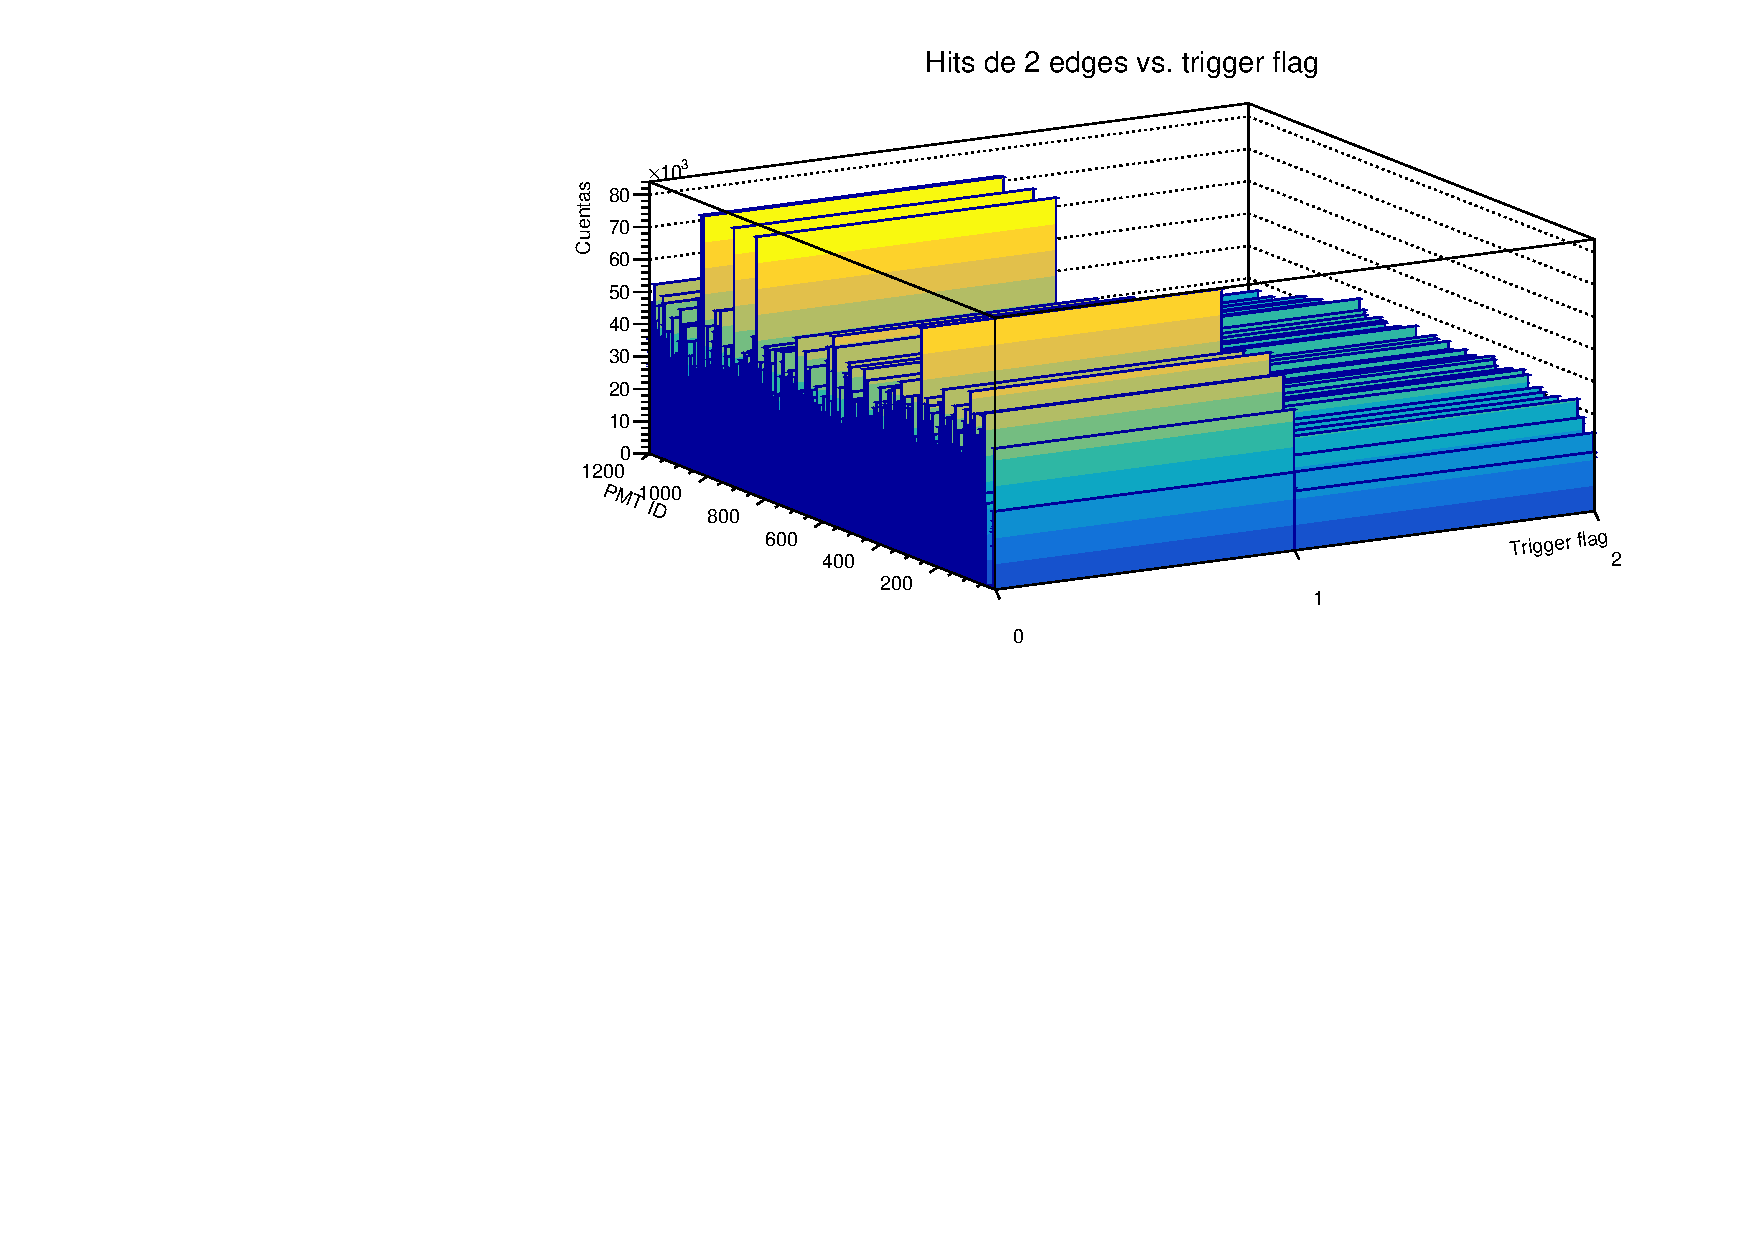
\includegraphics[width=0.55\textwidth]{../Figuras/Prob4Edge2}}\subfloat[Trigger flag vs. PMT ID para hits con 4 edges]{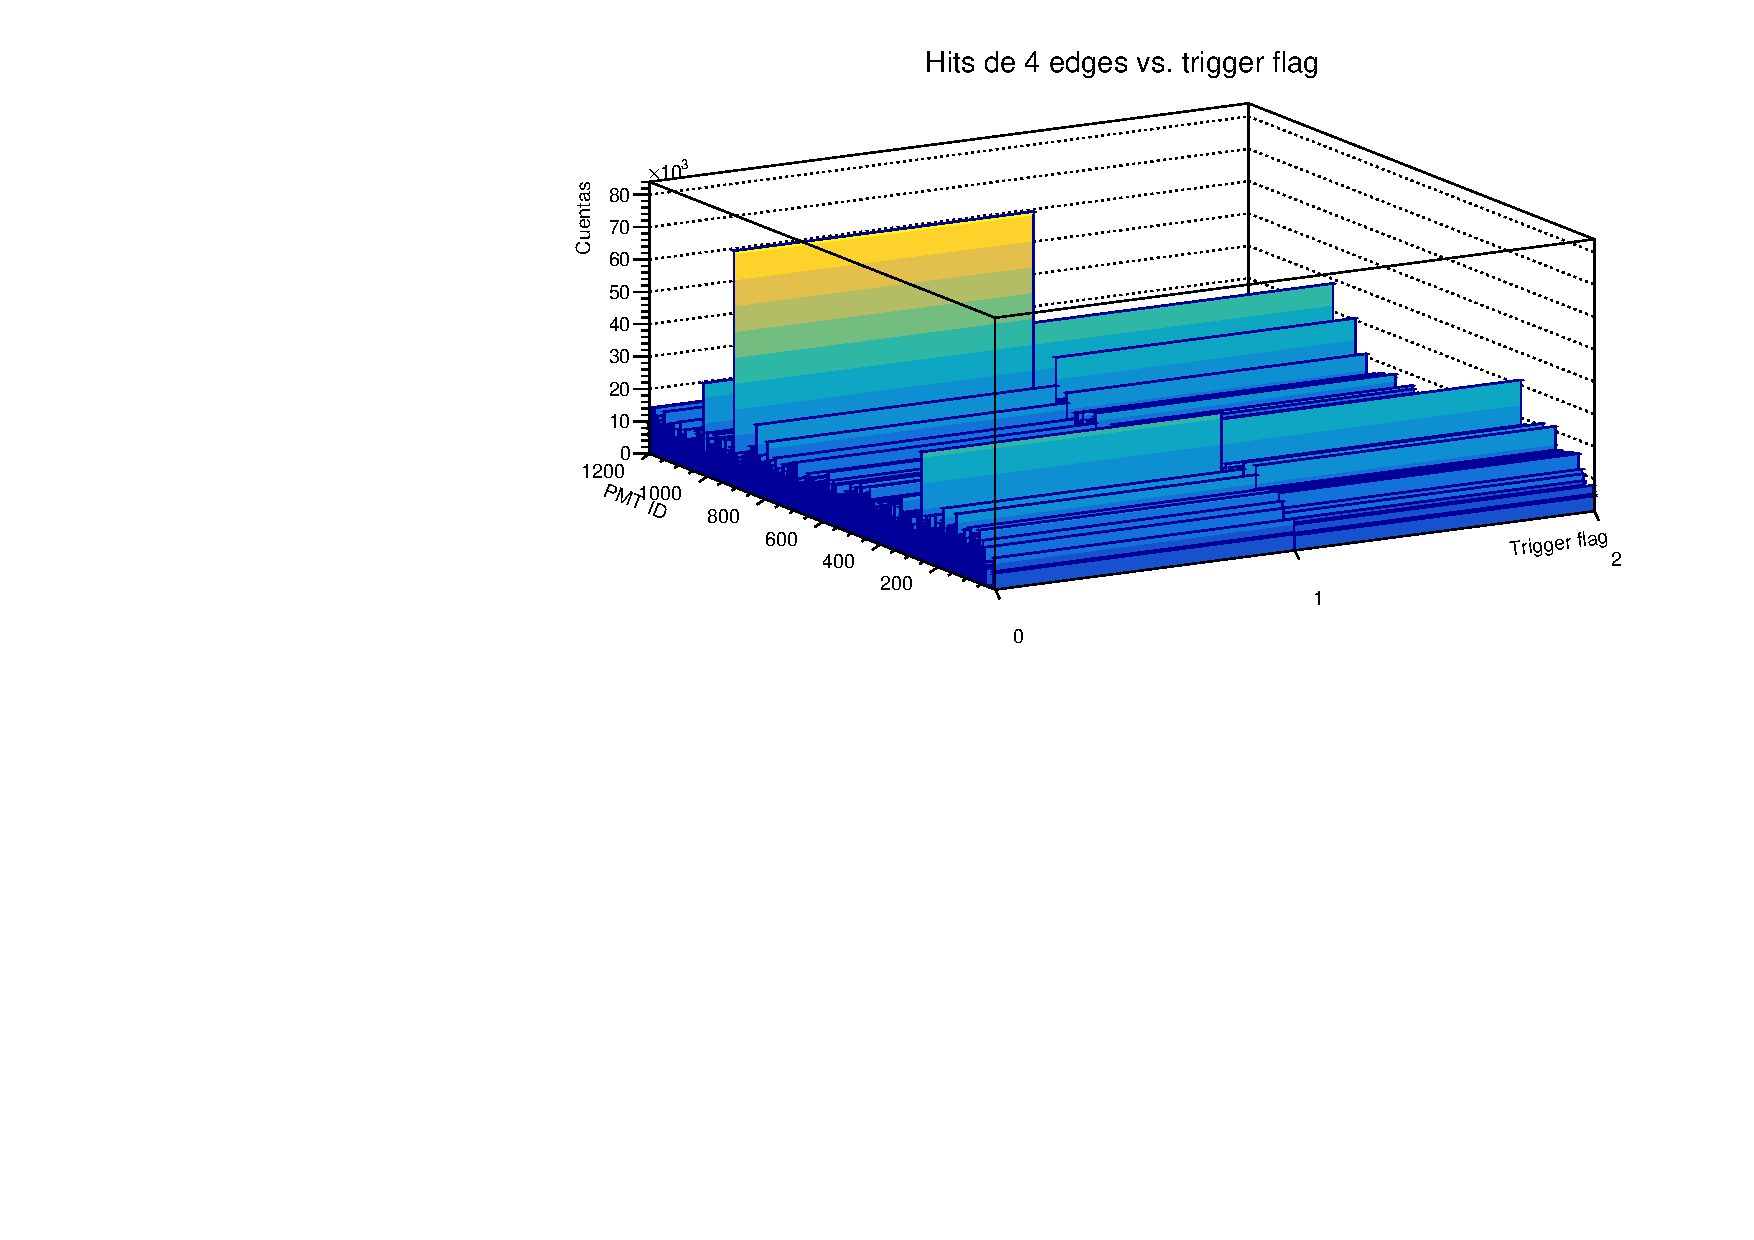
\includegraphics[width=0.55\textwidth]{../Figuras/Prob4Edge4}}

\subfloat[Trigger flag vs. PMT ID para hits con 2 y 4 edges]{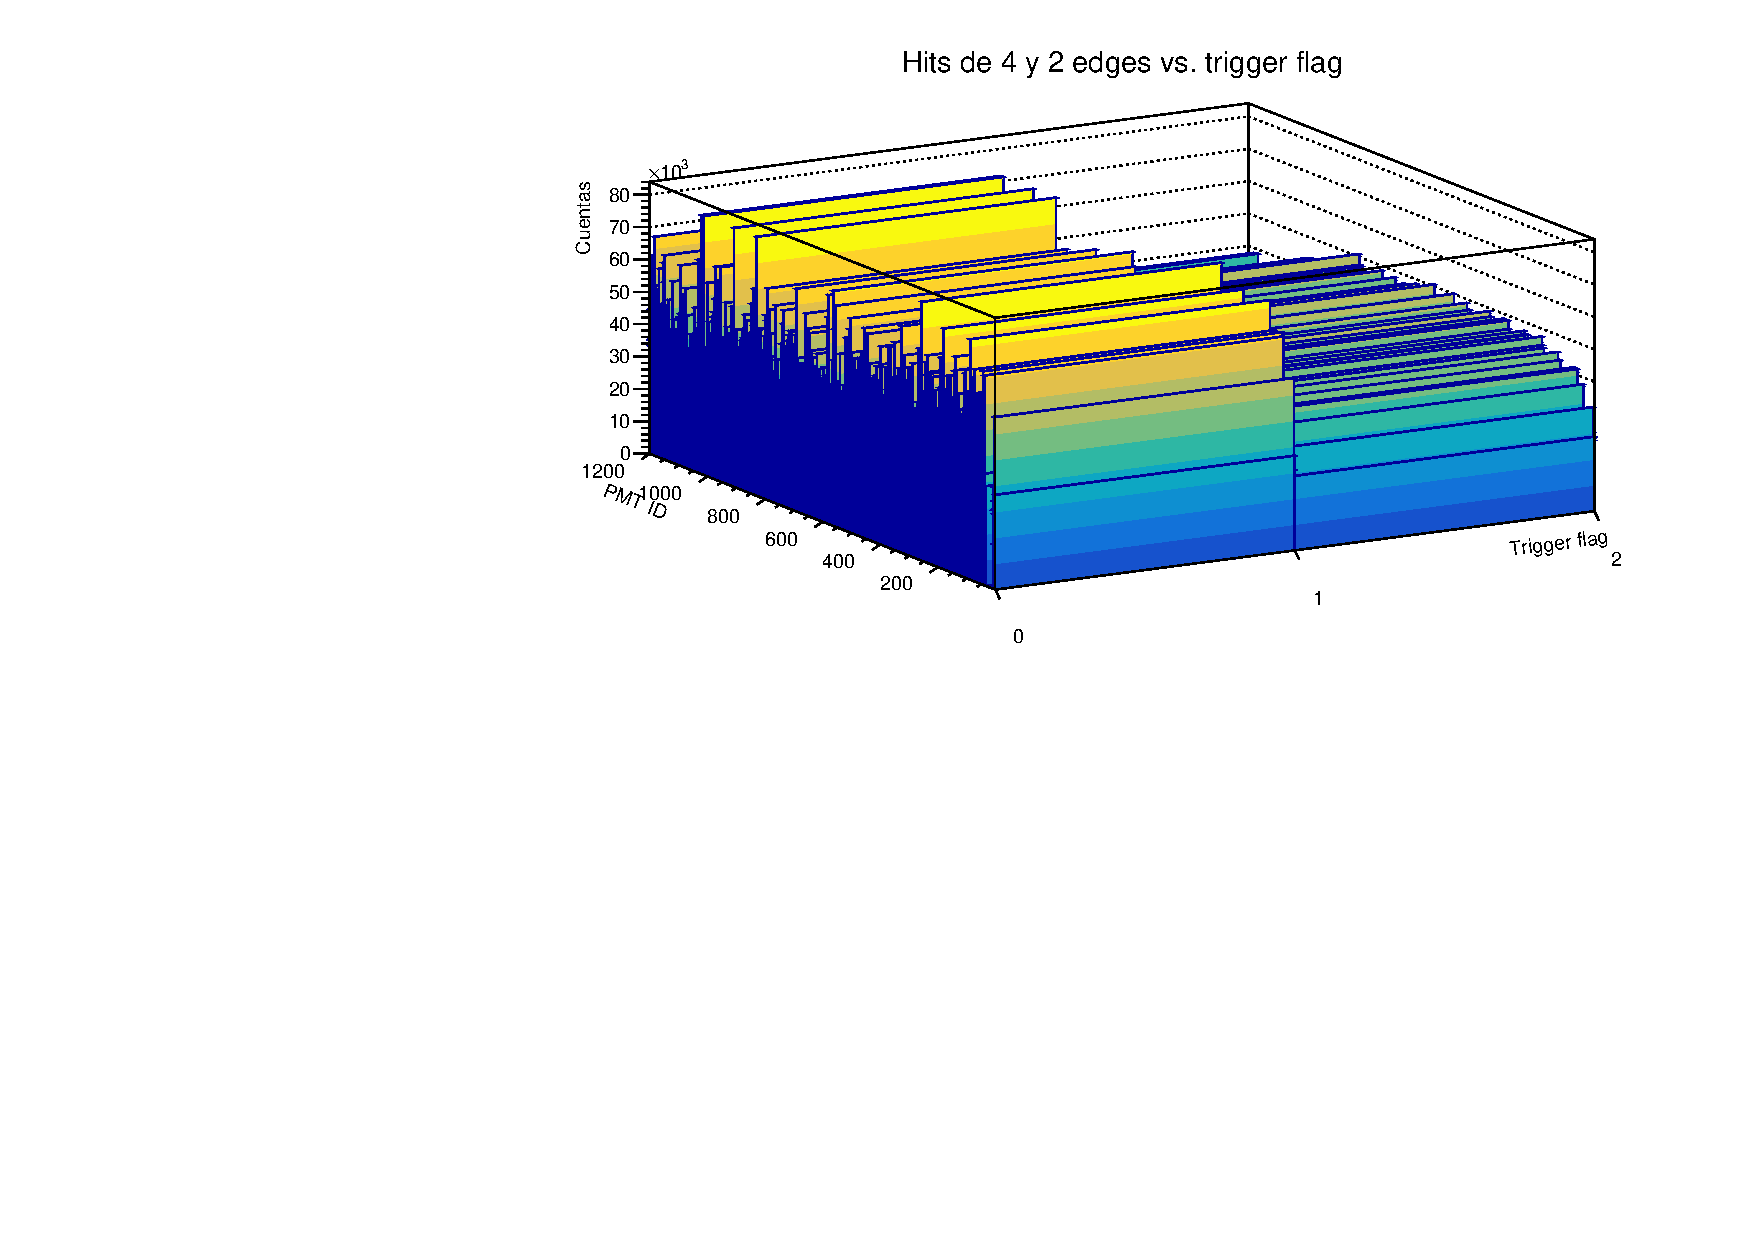
\includegraphics[width=0.55\textwidth]{../Figuras/Prob4Edge2y4}}
\caption{En los histogramas se muestra el número de hits, de 2 y 4 edges, que fueron usados para el trigger (trigger flag=1), así como el número de hits que no fueron usados para el trigger (trigger flag=0). En la figura (c) se muestra la combinación de ambos tipos de pulso.}
\label{fig:Prob4}
\end{figure}

Cuando trigger flag es igual a 1 quiere decir que el hit entró en el trigger. En la figura \ref{fig:Prob4} (a), se observa que hay más eventos que no fueron seleccionados para el trigger, mientras que en la figura \ref{fig:Prob4} (b) el número de eventos usados en el trigger aumenta significativamente. Sin embargo, si se aprecia con cuidado las figuras \ref{fig:Prob4} (a) y (b), es posible observar que, en promedio, el número de hits de 2 edges que entran en el trigger es del orden de $30\times 10^3$, mientras que para hits de 4 edges es del orden de $20\times 10^3$, por lo cual se sugiere que los pulsos pequeños parecen participar más en el trigger. No obstante, lo que comentamos no es válido en general, ya que hay PMT en los que hay más hits de 4 edges que participan en el trigger, que hits de 2 edges. 



\end{document}